\section{Randonnée}
\ifprof
\else
Lors d'une randonnée, un promeneur active son GPS pour retracer son parcours. Chaque point de mesure est caractérisé par quatre informations : la latitude (en degrés), la longitude (en degrés), l'altitude (en mètres) et le temps (en secondes). 
Ces informations sont stockées dans 4  tableaux :

\noindent \texttt{lat = [45.461516, 45.461448, 45.461383, 45.461641, 45.461534, 45.461595, 45.461562, ...]}

\noindent \texttt{long = [6.44461, 6.444426, 6.444239, 6.444035, 6.443879, 6.4437, 6.443521, ...]}

\noindent \texttt{alt = [1315.221, 1315.702, 1316.182, 1316.663, 1317.144, 1317.634, 1318.105, ...]}

\noindent \texttt{tps = [1597496965, 1597496980, 1597496995, 1597496710, 1597496725, 1597496740, 1597496755, ...]}.

\fi

\subsection{Analyse du profil global}



\question{Donner l'instruction permettant de connaître la taille du tableau \texttt{lat}.}
\ifprof
\begin{corrige}~\\
\vspace{-.5cm}
\begin{lstlisting}
>>> len(lat)
\end{lstlisting}
\end{corrige}
\else
\fi

Le module \texttt{math} fournit la fonction \texttt{radians} qui convertit des degrés en radians.


\question{Implémenter la fonction \texttt{conversion(L:list)-> list} permettant de convertir chacune des valeurs d'un tableau de flottants en radians. Cette fonction agira sans effet de bord.}
\ifprof
\begin{corrige}~\\
\vspace{-.5cm}
\begin{lstlisting}
def conversion(L:list) -> list : 
    tab = []
    for el in L : 
        tab.append(m.radians(el))
    return tab
\end{lstlisting}
\end{corrige}
\else
\fi

\question{Donner les instructions permettant de créer les tableaux \texttt{latr} et \texttt{longr}, résultats de la conversion en radians des tableaux \texttt{lat} et \texttt{long}.}
\ifprof
\begin{corrige}~\\
\vspace{-.5cm}
\begin{lstlisting}
>>> latr = conversion(lat)
>>> longr = conversion(long)
\end{lstlisting}
\end{corrige}
\else
\fi

\question{Implémenter la fonction \texttt{plus\_haut(L:list) -> float} permettant de déterminer l'altitude la plus haute atteinte lors de la randonnée (la fonction \texttt{max} sera ici interdite).}
\ifprof
\begin{corrige}~\\
\vspace{-.5cm}
\begin{lstlisting}
def plus_haut(L:list) -> float :
    maxi = L[0]
    for el in L : 
        if el>maxi :
            maxi = el  
    return maxi
\end{lstlisting}
\end{corrige}
\else
\fi

\question{Implémenter la fonction \texttt{plus\_haut\_indice(L:list) -> float} permettant de déterminer l'indice de l'altitude la plus haute atteinte lors de la randonnée.}
\ifprof
\begin{corrige}~\\
\vspace{-.5cm}
\begin{lstlisting}
def plus_haut_indice(L:list) -> float :
    m = 0
    for i in range(len(L)):
        if L[i]>L[m] :
            m = i  
    return m
\end{lstlisting}
\end{corrige}
\else
\fi

\question{En utilisant la fonction précédente, implémenter la fonction \texttt{coords\_plus\_haut(alt:list, long:list, lat:list)-> list} permettant de renvoyer la liste \texttt{[latitude, longitude]} des coordonnées du point le plus haut de la randonnée.}
\ifprof
\begin{corrige}~\\
\vspace{-.5cm}
\begin{lstlisting}
def coords_plus_haut(alt:list, long:list, lat:list)-> list :
    m = plus_haut_indice(alt)
    return[lat[m],long[m]]
\end{lstlisting}
\end{corrige}
\else
\fi

\question{Implémenter la fonction \texttt{deniveles(alt:list) -> list} qui calcule les dénivelés cumulés positif et négatif (en mètres) de la randonnée, sous forme d’une liste de deux flottants. Le dénivelé positif est la somme des
variations d’altitude positives sur le chemin, et inversement pour le dénivelé négatif.}
\ifprof
\begin{corrige}~\\
\vspace{-.5cm}
\begin{lstlisting}
def deniveles(alt:list) -> list:
    pos,neg = 0,0
    for i in range(1,len(alt)) : 
        delta = alt[i]-alt[i-1]
        if  delta > 0: 
            pos = pos + delta
        else : 
            neg = neg + delta
    return [pos,neg]
\end{lstlisting}
\end{corrige}
\else
\fi

\ifprof
\else
\vspace{.25cm}

Nous avons à notre disposition la fonction \texttt{distance(list:c1, list:c2) -> float} permettant de déterminer la distance entre deux points successifs en tenant compte de la latitude, de longitude, de l'altitude d'un point~1 de coordonnées \texttt{c1} et d'un point~2 de coordonnées \texttt{c2}, du rayon de la Terre \textit{etc}. \texttt{c1} est constitué de l'altitude, la latitude et la longitude d'un seul point.
\fi

\question{Implémenter la fonction \texttt{distance\_totale(alt:list, long:list, lat:list) -> float} renvoyant la distance parcourue (en mètres) au cours de la randonnée.}
\ifprof
\begin{corrige}~\\
\vspace{-.5cm}
\begin{lstlisting}
def distance_totale(alt:list, long:list, lat:list)-> float :
    D = 0
    for i in range(1,len(alt)):
        c1  = [alt[i-1],lat[i-1],long[i-1]]
        c2  = [alt[i],lat[i],long[i]]
        D = D + distance(c1,c2)
    return D
\end{lstlisting}
\end{corrige}
\else
\fi


\ifprof
\else
\newpage
\fi

\subsection{Découpage du profil}

\ifprof
\else
Dans cette partie, nous allons chercher à découper le profil de la randonnée en tentant de retrouver les différentes montagnes franchies par le randonneur.

\begin{figure}[H]
\centering
\includegraphics[width=.6\linewidth]{programmes/fig_01}
\caption{Profil de la randonnée}
\end{figure}
\fi

\question{Implémenter la fonction \texttt{moyenne(alt:list) -> float} permettant de calculer la moyenne des altitudes mesurées par le GPS.}
\ifprof
\begin{corrige}~\\
\vspace{-.5cm}
\begin{lstlisting}
def moyenne(alt:list):
    somme = 0
    for a in alt : 
        somme = somme + a
    return somme/len(alt)
\end{lstlisting}
\end{corrige}
\else
\fi

\ifprof
\else
\vspace{.5cm}

On note PND les points de passages par le niveau moyen en descente et PNM les points de passage par le niveau moyen en montée. 

\begin{figure}[H]
\centering
\includegraphics[width=.6\linewidth]{programmes/fig_03}
\caption{Points de passage par le niveau moyen en montée [PNM]}
\end{figure}
\fi

\question{Implémenter la fonction \texttt{indice\_premier\_PNM(alt:list) -> int} renvoyant, s’il existe, l’indice \texttt{i}
du premier élément de la liste tel que cet élément soit inférieur à la moyenne et l’élément suivant
soit supérieur à la moyenne. Cette fonction devra renvoyer \texttt{-1} si aucun élément vérifiant cette
condition n’existe.}
\ifprof
\begin{corrige}~\\
\vspace{-.5cm}
\begin{lstlisting}
def indice_premier_PNM(alt:list):
    m = moyenne(alt)
    indice = -1
    for i in range(len(alt)-1):
        if alt[i]<m and alt[i+1]>m:
            return i
    return indice
\end{lstlisting}
\end{corrige}
\else
\fi

\question{Implémenter la fonction \texttt{indices\_PNM(alt:list) -> list} retournant la liste des indices de tous les PNM.}
\ifprof
\begin{corrige}~\\
\vspace{-.5cm}
\begin{lstlisting}
def indices_PNM(alt:list):
    m = moyenne(alt)
    les_PNM = []
    for i in range(len(alt)-1):
        if alt[i]<m and alt[i+1]>m:
            les_PNM.append(i)
    return les_PNM
\end{lstlisting}
\end{corrige}
\else
\fi


\question{Dans le but de séparer les différents profils, nous allons chercher les indices des altitudes minimales entre deux PNM successifs. Implémenter la fonction \texttt{liste\_alt\_mini(alt:list) -> list} qui répond à ce besoin.}
\ifprof
\begin{corrige}~\\
\vspace{-.5cm}
\begin{lstlisting}
def liste_alt_min(alt:list):
    les_PNM = indices_PNM(alt)
    les_min = []
    for i in range(len(les_PNM)-1):
        mini = les_PNM[i]
        for j in range(les_PNM[i],les_PNM[i+1]):
            if alt[j]<alt[mini]:
                mini = j
        les_min.append(mini)
    return les_min
\end{lstlisting}
\end{corrige}
\else
\fi

\ifprof
\else
On appelle \texttt{pam} la liste des indices des points ayant une altitude minimale.

\begin{figure}[H]
\centering
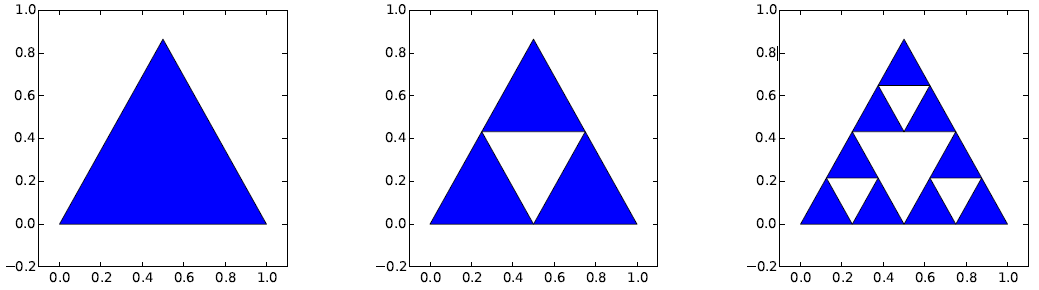
\includegraphics[width=.6\linewidth]{programmes/fig_04}
\caption{Points avec altitude minimale [pam]}
\end{figure}

On souhaite maintenant décomposer le profil mesuré en plusieurs << montagnes >>. 
Une montagne est une liste constituée d'altitudes successives.
La première montagne ira de la première altitude mesurée au premier \texttt{pam}. 
On aura ensuite une montagne entre chaque \texttt{pam}. 
La dernière montagne ira du dernier \texttt{pam} à la dernière altitude mesurée.
\fi


\question{Implémenter la fonction \texttt{creer\_montagnes(alt) -> list} renvoyant une liste constituée de la liste des montagnes élémentaires.}
\ifprof
\begin{corrige}~\\
\vspace{-.5cm}
\begin{lstlisting}
def creer_montagnes(alt):
    pam = liste_alt_min(alt)
    montagnes = []
    mont = []
    for i in range(0,pam[0]):
        mont.append(alt[i])
    montagnes.append(mont)
    for i in range(len(pam)-1):
        mont = []
        for j in range(pam[i],pam[i+1]):
            mont.append(alt[j])
        montagnes.append(mont)
    mont = []
    for i in range(pam[-1],len(alt)):
        mont.append(alt[i])
    montagnes.append(mont)
    return montagnes
\end{lstlisting}
\end{corrige}
\else
\fi


\ifprof
\else
\begin{figure}[H]
\centering
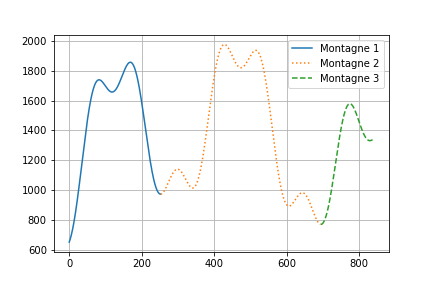
\includegraphics[width=.6\linewidth]{programmes/fig_05}
\caption{Découpage en montagnes}
\end{figure}
\fi

%
%
%
%%% TO DO RECHERCHE DU SECOND MAXIMUM
%%% 
%
%
%\section{Marche auto-évitante}
%
%
%Une marche auto-évitante est un processus au cours duquel un point décrit un chemin auto-évitant, c’est-à-dire
%qui ne se recoupe jamais lui-même. Ce modèle peut servir lors de la modélisation d’une chaîne polymère.
%En effet, deux monomères distincts de la chaîne ne peuvent pas se trouver à deux positions identiques pour
%des raisons d’encombrement stérique.
%
%Dans ce sujet, on appellera chemin auto-évitant (CAE) de longueur $n$ tout ensemble de $n+1$ points $P_i \in \mathbb{Z}^2$ pour $0\leq i \leq n$ tels que : 
%\begin{itemize}
%\item $\forall i, ||P_{i+1}-P_i|| = 1$;
%\item $\forall (i,j); i\neq j \Rightarrow P_i \neq P_j$.
%\end{itemize}
%
%
%Chaque point du chemin sera représenté par une liste à deux éléments entiers précisant les deux coordonnées
%(par exemple $P_i = (5;4)$ est représenté par la liste \texttt{[5,-4]}). Le chemin lui-même est constitué de la liste
%des points, dans l’ordre dans lequel ils sont atteints. Les codes Python produits dans cette partie devront
%manipuler exclusivement des coordonnées entières.
%
%Voici un exemple de représentation graphique de CAE de longueur 30 à partir de $(0; 0)$.
%
%\begin{figure}[H]
%\centering
%\includegraphics[width=.6\linewidth]{fig_01}
%\end{figure}
%
%On s’intéresse dans un premier temps à une méthode naïve pour générer un chemin auto-évitant de longueur
%$n$ sur une grille carrée. La méthode adoptée est une approche gloutonne :
%\begin{enumerate}
%\item le premier point est choisi à l’origine : $P_0 = (0; 0)$;
%\item en chaque position atteinte par le chemin, on recense les positions voisines accessibles pour le pas
%suivant et on en sélectionne une au hasard. En l’absence de positions accessibles l’algorithme échoue;
%\item on itère l’étape 2 jusqu’à ce que le chemin possède la longueur désirée ou échoue.
%\end{enumerate}
%
%Le module \texttt{random} fournit la fonction \texttt{randrange(a, b)} qui renvoie un entier compris entre $a$ et $b-1$
%inclus, ainsi que la fonction \texttt{choice(L)} qui renvoie l’un des éléments de la liste \texttt{L}, dans les deux cas choisis
%aléatoirement avec une probabilité uniforme.
%
%L’expression \texttt{x in L} est une expression booléenne qui vaut \texttt{True} si \texttt{x} est l’un des éléments de \texttt{L} et \texttt{False} dans le cas contraire. On supposera que la méthode employée pour évaluer cette expression sur une liste est une recherche séquentielle.
%La valeur spéciale \texttt{None} est utilisée en Python pour représenter une valeur invalide, inconnue ou indéfinie.
%L’expression booléenne \texttt{v is None} indique si la valeur de \texttt{v} est cette valeur spéciale.
%
%
%*******En utilisant le canevas fourni en annexe et en ajoutant les import nécessaires :********
%
%\question{Soit un point $P$ de coordonnées $(0,0)$, donner les coordonnées des points voisin de ce point.}
%\ifprof
%\begin{corrige}
%Les points voisins sont de coordonnées $(1,0)$, $(0,1)$, $(-1,0)$ et $(0,-1)$.
%\end{corrige}
%\else
%\fi\question{Soit un point $P$ de coordonnées $(x,y)$ (en Python, le point \texttt{p} sera modélisé par une liste de ses coordonnées : \texttt{[x,y]}), donner les coordonnées des points voisin de ce point.}
%\ifprof
%\begin{corrige}
%Les points voisins sont de coordonnées $(x+1,y)$, $(x,y+1)$, $(x-1,y)$ et $(x,y-1)$ soit en python \texttt{[x+1,y]}, \texttt{[x,y+1]}, \texttt{[x-1,y]} et \texttt{[x,y-1]}.
%\end{corrige}
%\else
%\fi
%
%
%\question{Implémenter la fonction \texttt{voisins(p:list) -> list} qui construit la liste des positions
%voisines de~\texttt{p}.}
%\ifprof
%\begin{corrige}~\\
%\vspace{-.5cm}
%\begin{lstlisting}
%def voisins(p:list) -> list :
%    x = p[0]
%    y = p[1]
%    v = [[x+1,y],[x,y+1],[x-1,y],[x,y-1]]
%    return v
%\end{lstlisting}
%\end{corrige}
%\else
%\fi
%
%\question{Implémenter la fonction \texttt{positions\_possibles(p:list, atteints:list)-> list} qui construit la liste des positions
%suivantes possibles à partir du point \texttt{p}. La liste atteints contient les points déjà atteints par le chemin.}
%\ifprof
%\begin{corrige}~\\
%\vspace{-.5cm}
%\begin{lstlisting}
%def positions_possibles(p:list, atteints:list)-> list :
%    possibles = []
%    voi = voisins(p)
%    for v in voi : 
%        if v not in atteints: 
%            possibles.append(v)
%    return possibles
%\end{lstlisting}
%\end{corrige}
%\else
%\fi
%
%\question{Mettre en évidence graphiquement un exemple de CAE le plus court possible pour lequel, à une
%étape donnée, la fonction  \texttt{positions\_possibles} va renvoyer une liste vide. En prenant en compte les symétries,
%combien de tels chemins distincts existent pour cette longueur minimale ?}
%\ifprof
%\begin{corrige}~\\
%8 chemins.
%\end{corrige}
%\else
%\fi
%
%\question{Implémenter la fonction \texttt{genere\_chemin\_naif(n:int) -> list } qui construit la liste des points représentant le 
%chemin auto-évitant de longueur \texttt{n} et renvoie le résultat, ou bien renvoie la valeur spéciale \texttt{None} si à une
%étape \texttt{positions\_possibles} renvoie une liste vide.}
%\ifprof
%\begin{corrige}~\\
%\vspace{-.5cm}
%\begin{lstlisting}
%def foo:
%    return bar
%\end{lstlisting}
%\end{corrige}
%\else
%\fi
%Une personne curieuse et patiente a écrit le code suivant.
%
%\begin{lstlisting}
%from chemin import genere_chemin_naif
%
%N, M, L, P = 10000, 351, [], []
%
%for n in range(1, M):
%    nb = 0
%    for i in range(N):
%        chemin = genere_chemin_naif(n)
%            if chemin is None:
%                nb += 1
%    L.append(n)
%    P.append(nb / N)
%
%import matplotlib.pyplot as plt
%plt.plot(L, P)
%plt.grid()
%plt.show()
%\end{lstlisting}
%
%Après un long moment, elle a obtenu le graphique suivant, volontairement laissé sans étiquettes d’axes.
%
%\begin{figure}[H]
%\centering
%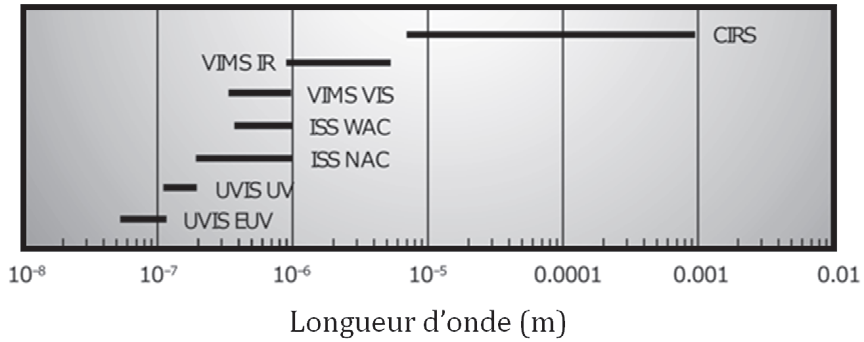
\includegraphics[width=.6\linewidth]{fig_02}
%\end{figure}
%
%\question{Décrire ce que représente ce graphique et interpréter sa signification pour la méthode naïve.}
%\ifprof
%\begin{corrige}~\\
%\vspace{-.5cm}
%\begin{lstlisting}
%def foo:
%    return bar
%\end{lstlisting}
%\end{corrige}
%\else
%\fi
%
%
%Afin d’éviter les inconvénients de la méthode précédente, on s’intéresse à une solution différente nommée
%méthode du pivot, proposée par Moti Lal en 1969. Son principe est le suivant :
%\begin{enumerate}
%\item on part d’un chemin auto-évitant arbitraire de longueur n. Ici, on choisira une initialisation très simple,
%le chemin droit \texttt{[ [0, 0], [1, 0], [2, 0], ..., [n, 0] ]};
%\item on sélectionne au hasard un point, nommé pivot, entre le second et l’avant-dernier point du chemin,
%et un angle aléatoire de rotation parmi $\pi$, $\dfrac{\pi}{2}$ et $-\dfrac{\pi}{2}$;
%\item on laisse les points avant le pivot inchangés et on fait subir à l’ensemble des points situés strictement
%après le pivot une rotation ayant pour centre le pivot et pour angle, l’angle choisi à l’étape 2 ci-dessus.
%\item si le chemin ainsi obtenu est auto-évitant, on le garde. Sinon, on reprend à l’étape 2 la sélection d’un
%pivot et d’un angle, jusqu’à en trouver une paire qui conviennent.
%\item on répète les étapes 2 à 4 un certain nombre de fois. Le choix du nombre minimal de rotations à
%effectuer pour obtenir un chemin non corrélé au chemin initial est laissé de côté dans ce sujet.
%\end{enumerate}
%
%Cette méthode permet de générer de manière efficace des marches auto-évitantes de plusieurs milliers de
%points, comme la marche ci-dessous de longueur 2000.
%
%\begin{figure}[H]
%\centering
%\includegraphics[width=.6\linewidth]{fig_03}
%\end{figure}
%
%Dans cet algorithme, une étape importante est la vérification qu’un chemin donné est auto-évitant. Pour
%vérifier cela on pourrait bien sûr s’y prendre comme dans la fonction \texttt{positions\_possibles}, mais on adopte
%une méthode différente avec une fonction \texttt{est\_CAE(chemin)} qui trie les points du chemin puis met à profit
%ce tri pour vérifier efficacement que le chemin est auto-évitant.
%
%On utilise pour cela la fonction \texttt{sorted} qui renvoie une nouvelle liste triée par ordre croissant. Elle fonctionne
%sur tout type d’éléments disposant d’une relation d’ordre, y compris des listes pour lesquelles l’ordre lexicographique
%(ordre du premier élément, en cas d’égalité du second, etc.) est appliqué. %On suppose de plus que
%%la complexité temporelle asymptotique dans le pire des cas de cette fonction est la meilleure possible.
%
%
%
%\question{Implémenter la fonction \texttt{est\_CAE(chemin)} qui vérifie si un chemin est auto-évitant en se basant sur sorted et renvoie un résultat booléen. Elle devra ne pas être de complexité temporelle asymptotique
%dans le pire des cas supérieure à la fonction \texttt{sorted} : vous prouverez ce dernier point.}
%\ifprof
%\begin{corrige}~\\
%\vspace{-.5cm}
%\begin{lstlisting}
%def foo:
%    return bar
%\end{lstlisting}
%\end{corrige}
%\else
%\fi
%
%
%\question{Implémenter la fonction \texttt{rot(p, q, a)} qui renvoie le point image du point \texttt{q} par la rotation de centre \texttt{p} et d’angle défini par la valeur de \texttt{a} : 0 pour $\pi$, 1 pour $\dfrac{\pi}{2}$, 2  pour
%$-\dfrac{\pi}{2}$.}
%\ifprof
%\begin{corrige}~\\
%\vspace{-.5cm}
%\begin{lstlisting}
%def foo:
%    return bar
%\end{lstlisting}
%\end{corrige}
%\else
%\fi
%
%\question{Implémenter la fonction \texttt{rotation(chemin, i\_piv, a)} qui renvoie un nouveau chemin identique à chemin jusqu’au pivot d’indice \texttt{i\_piv}, et ayant subi une rotation de a autour du pivot (même codage que
%la fonction précédente) sur la partie strictement après le pivot.}
%\ifprof
%\begin{corrige}~\\
%\vspace{-.5cm}
%\begin{lstlisting}
%def foo:
%    return bar
%\end{lstlisting}
%\end{corrige}
%\else
%\fi
%
%\question{Implémenter la fonction \texttt{genere\_chemin\_pivot(n, n\_rot)} permettant de générer un chemin autoévitant de longueur \texttt{n} en appliquant \texttt{n\_rot} rotations. L’application d’une rotation peut nécessiter plusieurs tentatives.}
%\ifprof
%\begin{corrige}~\\
%\vspace{-.5cm}
%\begin{lstlisting}
%def foo:
%    return bar
%\end{lstlisting}
%\end{corrige}
%\else
%\fi


%\question{On considère un pivot, son point précédent et son point suivant. Quel est l’impact prévisible sur les
%rotations admissibles ? Suggérer un moyen de prendre en compte cette propriété pour améliorer l’algorithme.}
%\ifprof
%\begin{corrige}~\\
%\vspace{-.5cm}
%\begin{lstlisting}
%def foo:
%    return bar
%\end{lstlisting}
%\end{corrige}
%\else
%\fi